\documentclass[a4paper,10pt]{article}
\usepackage[% bw,window,corporate
]{EPFL}
%\def\familydefault{\rmdefault}    % uncomment for serif fonts in body

\title{Graph Networks for Wind Nowcasting}
\subtitle{ Graph Networks offer a flexible way of handling non-regular dataset such as sparse measures in the 3D space.}
\author{Arnaud Pannatier}
\narrowmargins                    % uncomment for narrow margins
\symmetricmargins                 % uncomment for equal margins
\unitname{EDIC}{Idiap Research Institute}{Machine Learning Group}
\course{EE-452}{Network Machine Learning}
\usepackage{booktabs}       % professional-quality tables
\usepackage{multirow}
\usepackage{amsmath}
\usepackage{graphicx}
\usepackage{caption}
\usepackage{subcaption}
\usepackage{wrapfig}

\newcommand{\ap}[1]{\marginpar{{\tiny \color{red} [AP] #1}}}
\begin{document}

\maketitle

\section{Introduction}
Air Traffic Controllers (ATC) need to have access to reliable wind speed forecasts to organize the airspace efficiently. At cruising altitudes, the only measures that one has access to are measured by airplanes that record the wind along their trajectories, and fortunately, as there are a lot of planes flying in the airspace ATCs have recorded a lot of data. Their interest is to be able to a good prediction during the window of time they operate which is rather short (30min up to a few hours) In that range, called nowcasting, one gets the most accurate forecast by extrapolating from the latest measures available rather than trying to solve expensive numerical equations solvers.
It is in that range that deep learning methods can offer a lot, as meteorological data is often highly available. Sadly this data are recorded along trajectories and is sparse in space, so we cannot uses standard methods such as CNN to deal with it. We noticed that it could be a good candidate for Graph Networks are their inductive bias makes them good candidates for this task.

This work will use graph networks to forecast the wind speed at cruising altitudes. We will use the \textit{SkySoft ATM MALAT Wind Speed Dataset} \cite{skysoft2021dataset} and starting from an Graph Element Network (GEN) \cite{alet2019gen} implementation, we will analyse the effect of the topology of the graphs and different nodes and edge features on the performance of the model.



\subsection{Problem formulation}

Let $\mathbb{X}, \mathbb{I}, \mathbb{O}$ be three bounded metric spaces, and define two functions $f : \mathbb{X}\rightarrow \mathbb{I}$, mapping from data to the input space, and $g : \mathbb{X}\rightarrow \mathbb{O}$ mapping to the output space.
In the case of wind nowcasting, $\mathbb{X} = \mathbb{R}^{3} \times \mathbb{R}^{+}$, which corresponds to 3 spatial coordinates and one temporal and $\mathbb{I} = \mathbb{O} = \mathbb{R}^{2}$ which encode the wind in the $(x,y)$ plane.
We want to learn the transformation which maps a function $f$ to $g$.
We only have access to $f$ by data $(x, i)  \in \mathbb{X} \times \mathbb{I}$ of measures $i$ at position $x$ and we know $g$ only through a set $(x', o) \in \mathbb{X} \times \mathbb{O}$ of measurements $o$ at position $x'$.
So we learn this mapping from data using multiple sets of meaures corresponding to many $(f,g)$ pairs with the objective of minimizing the distance in the output metric space $\mathbb{O}$ between predictions and references.

\section{Related works}


\subsection{Graph Element Networks (GENs)} \label{ssec:gen}
Graph Element Networks \cite{alet2019gen} aim to model field transformations using a non-regular graphs with nodes in the underlying space $\mathbb{X}$. Each measurement $(x, i)$ is encoded using a small MLP, the initial latent feature of one node is then computing by averaging the embeddings of the measurements based on their distance to the node. The model then process this latent variable using $T \in \mathbb{N}$ steps of message passing, using the following equations:

\begin{align}
  m_{ij}^{t + 1} = m_e(l_{i}^{t}, l_{j}^{t}) \\
  l_{j}^{t + 1} = m_{n}(l_{i}^{t}, \sum_{(i,j) \in \mathcal{N}} m_{ij}^{t + 1})
\end{align}

Where $m_e, m_n$ are multilayer perceptrons and $l_{i}^{t}$ is the latent state of nodes $i$ at the $t$-th step of message passing. In that representation no edge features are used.
In order to predict a value at a new query position, the model linearly extrapolates in latent space, and decodes using a small MLP modelling the transformation from latent to output space.

\begin{figure}[htbp]
  \centering
  \includegraphics[width=\textwidth]{GEN}
  \caption{GEN architecture. The measures are first encoded to a latent space, then the initial node feature is computed by aggregate the closer encoded measures, processing is done by message passing and the final measures are retrieved by first interpolating the nodes features at the query position and then decoding.}
\end{figure}

\ap{advantages -- drawbacks}

\subsection{Finite Element Networks}

Traditional PDEs solvers are model the domain using regular grids, but this has some drawbacks as some part of the space might be more complicated to model than the other. One way of dealing with this problem is to use a Finite Element method approach \cite{hughes2012finite}, which uses a non-regular graph that can be denser in the more complex regions and coarser in the smoother regions.

\ap{advantages --drawbacks}


\section{Exploration}
% (30 points)
% The goal of this section is to analyze the data, and get insights about the tools that will help in the learning section: what handcrafted features could be useful? If you use graph neural networks, what parametrization should be used?

\subsection{Graph Types}
%     \item global properties of the graph (e.g., connected components, sparsity, diameter, clusters, degree distribution, spectrum)
%     \item the type of graph (e.g., power law, small world, regular, sampled manifold)
%     \item properties of the nodes (e.g., clustering coefficient, modularity, centrality)

Usually the mesh for FEM simulations is created beforehand with denser region where we expect the field to behave more complicated way. Meshes for this simulation are usually a triangulation of the region of interest. The triangulation subdivise the space into non overlapping triangles, such that each triangle have either a side or a vertex in common or are disjoint. A density parameter define the finess of the triangulation. The graph generated by such this triangulation scheme is such that there is an edge between two nodes only if there are close in the euclidean sense. The degree distribution of these graphs has only small values corresponding to the local neighborhood.

\begin{wrapfigure}{l}{5.5cm}
  \centering
  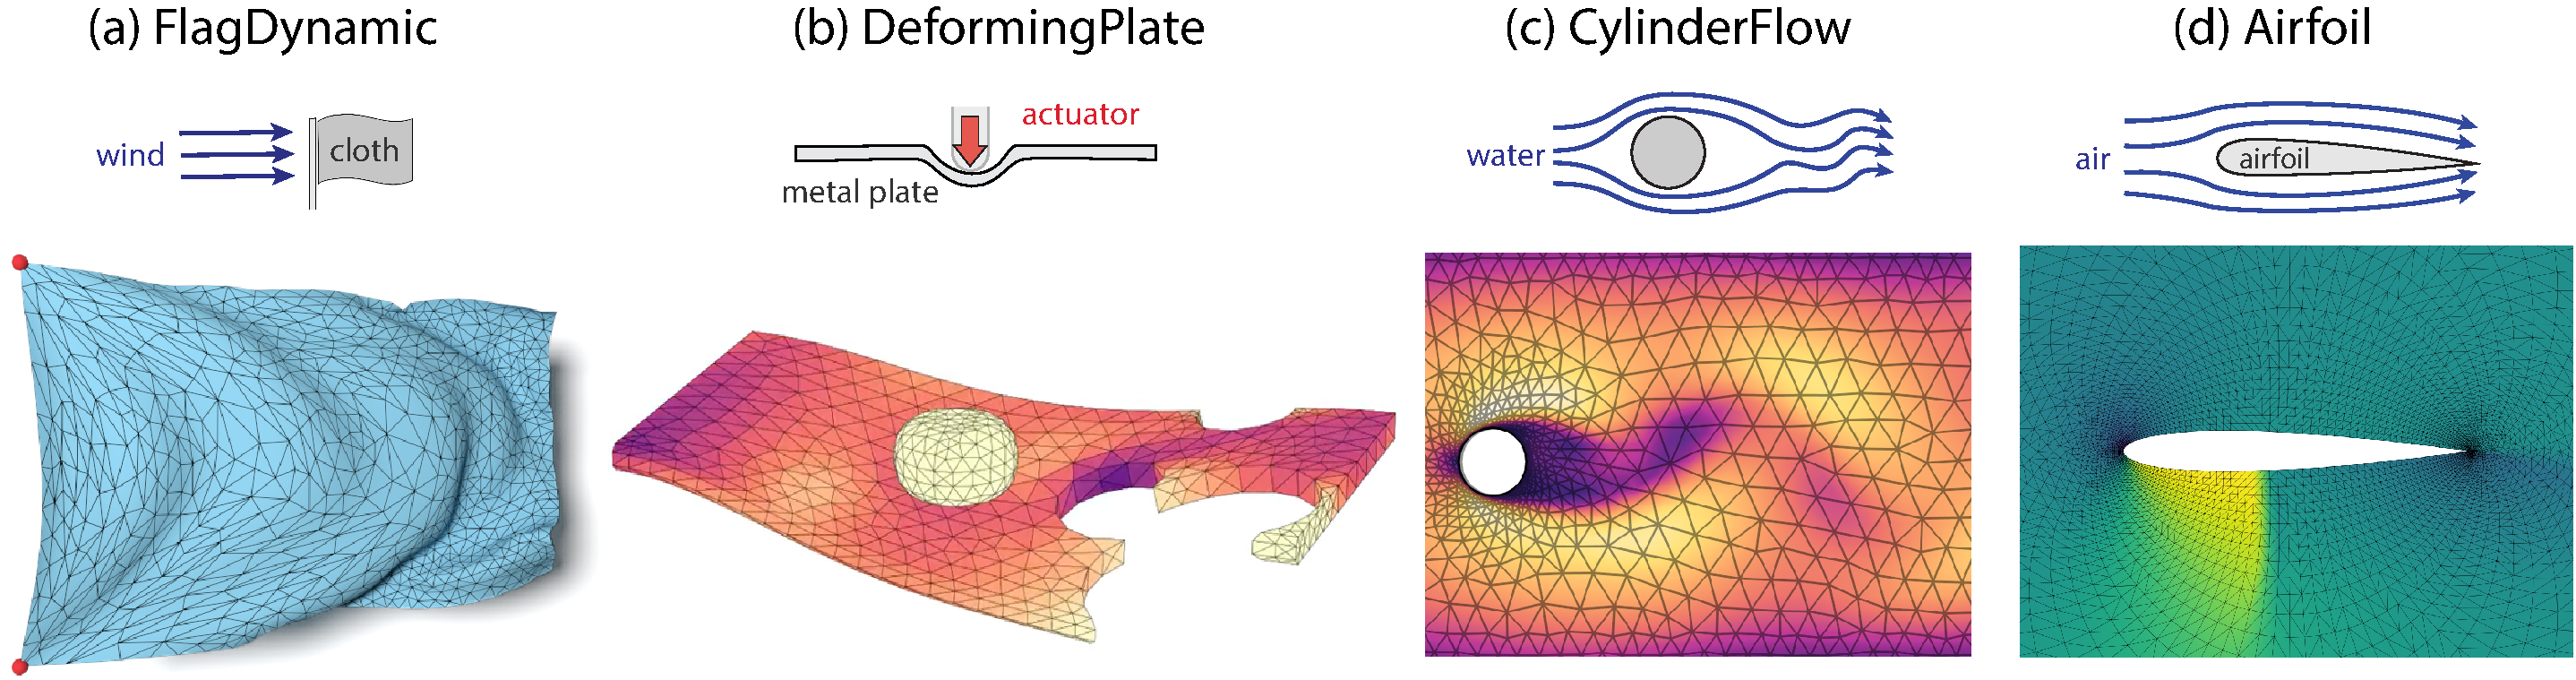
\includegraphics[trim={780 0 300 50},clip,width=0.3\textwidth]{mesh-dataset}
  \caption{Typical FEM meshing \cite{pfaff2020learning}}
\end{wrapfigure}

For GENs, the original way of creating graphs is to create a grid mesh that covers the whole space, and to encode the node position as parameters of the model, so that it can be optimized by gradient descent during training. In that case, the graph structure remains similar to the initial grid structure.

\ap{TODO : graph}

In both apporaches, only those graph structures have been used. In this work, we will consider three approaches for our graph topology. The first one, considered as baseline is constructed as follow : First we will take the $k$-means of the measure positions and we will add edges between the nearest neighbors. The second one will be a random network were the nodes position and their edges are taken at random, we will try different parameters $p$ and analyse its effect on the quality of the model.

For the last graph structure, we will use a Barab\'asi-Albert model scheme for growing a graph to a given number of nodes, we will then associate to each node one of the $k$-means position.
\ap{TODO : graph}


\subsection{Features}

In this work we will focus on nodes and edges features as we are using the graph network to do regression over the whole space. We won't need to aggregate the features over the whole graph.


\subsection{Nodes features}
As described in section~\ref{ssec:gen}, GEN are only using nodes features that are computed by aggregating the learned embeddings of the measures based on their distance. We will visualise their value in some very unbalanced cases and the effect of message passing on the features. This will help us to choose the message passing steps and guide us through the analysis of the different graph structures.

We assume that this part is the most important to get a good model. So we will explore different strategies and measure their impact on the model. First we will try to use no encoder and aggregate the normalized measured values. With this approach, we delegate the whole processing to the graph networks, and we think this should be already a strong baseline as the outputs values are strongly related to these initial values. We will then try to use fixed sine-cosine positional encodings ~\cite{vaswani2017attention} and 3D positional fixed sine-cosine positional encodings ~\cite{chu2021conditional}.

\subsection{Edge features}
A contribution of this work is to add edge features to GENs. We think that a good graph networks for space modelling should be able to compute approximation of the derivatives of values in the graph. We will take Euler scheme as an inspiration and have an explicit design for edge features that allows this kind of computation. We will make an ablation with learned features and see their effect on the quality of the model.
\ap{TODO: sketch}


Euler equation:

\begin{equation}
  \rho \mathbf{g} - \nabla p = \rho\frac{d\mathbf{v}}{dt}
\end{equation}


% You are free to use the tools that you want. We list below some examples of properties that you can analyze:
% \begin{itemize}
%     \item analysis of the attributes (e.g., their distribution, smoothness, graph Fourier transform). If the task is classification, are the labels balanced?
%     \item clustering (spectral clustering, $k$-means)
% \end{itemize}
% Vizualizations of the network may be very helpful
\section{Exploitation}

\subsection{Graph Types}

\begin{table*}
  \centering
  \begin{tabular}{lcccc} \toprule
    \multirow{2}{*}{\textbf{Model}}                      &                            & \multicolumn{3}{c}{\textbf{Nodes}}                                                           \\ \cmidrule(lr){3-5}
                                                         &                            & 10                                 & 100                    & 1000                           \\ \hline
    \multirow{2}{*}{\textbf{Random Network, $p=1\%$} }   & \scriptsize \textsc{Fixed} & 0.80  \tiny $\pm$ 0.04             & 0.71  \tiny $\pm$ 0.02 & 0.70 \tiny $\pm$ 0.02          \\
                                                         & \scriptsize \textsc{Adapt} & 0.69 \tiny $\pm$ 0.01              & 0.65 \tiny $\pm$ 0.02  & \textbf{0.64 \tiny $\pm$ 0.02} \\
    \multirow{2}{*}{\textbf{Random Network, $p=10\%$}}   & \scriptsize \textsc{Fixed} & 0.76  \tiny $\pm$ 0.03             & 0.70  \tiny $\pm$ 0.02 & 0.76 \tiny $\pm$ 0.02          \\
                                                         & \scriptsize \textsc{Adapt} & 0.69 \tiny $\pm$ 0.01              & 0.66 \tiny $\pm$ 0.01  & 0.66 \tiny $\pm$ 0.02          \\
    \multirow{2}{*}{\textbf{$k$-means, 3 nn.}          } & \scriptsize \textsc{Fixed} & 0.68  \tiny $\pm$ 0.01             & 0.69  \tiny $\pm$ 0.02 & 0.68 \tiny $\pm$ 0.01          \\
                                                         & \scriptsize \textsc{Adapt} & 0.68 \tiny $\pm$ 0.01              & 0.66 \tiny $\pm$ 0.01  & 0.65 \tiny $\pm$ 0.01          \\
    \multirow{2}{*}{\textbf{$k$-means, BA}             } & \scriptsize \textsc{Fixed} & 0.69  \tiny $\pm$ 0.01             & 0.68  \tiny $\pm$ 0.01 & 0.66 \tiny $\pm$ 0.02          \\
                                                         & \scriptsize \textsc{Adapt} & 0.68 \tiny $\pm$ 0.02              & 0.65 \tiny $\pm$ 0.02  & \textbf{0.64 \tiny $\pm$ 0.01} \\

    \bottomrule
  \end{tabular}
  \caption{
    We tried different graph topology for our model that use no embeddings. First, as a baseline, we tried Random Networks, were the position of each nodes is drawn from $\mathcal{U}(-1,1)$ and where there is an edge between two nodes with probability $p$. Then we tried to use $k$-means to get the position of the nodes and added edges either between the 3 nearest neighbors in the graph or following a Barabasi-Albert procedure. The results are the MSE error on the validation set, we ran ten different seeds to get the standard deviation. all measures are normalized.
  }
  \label{tab:graphs}
\end{table*}

The performance of the different graph types are displayed in Table \ref{tab:graphs}.
We see that allowing position to move during training (\textsc{Adapt} in the table) are always performing better than their fixed counterpart. Random Graphs are the baseline and we expect them to perform poorly as they are initialized randomly without taking into account additional insight that we can have about the dataset. We see that indeed their performance is worse than the other models.

\begin{figure}[htbp]
  \begin{subfigure}{0.24\textwidth}
    \centering
    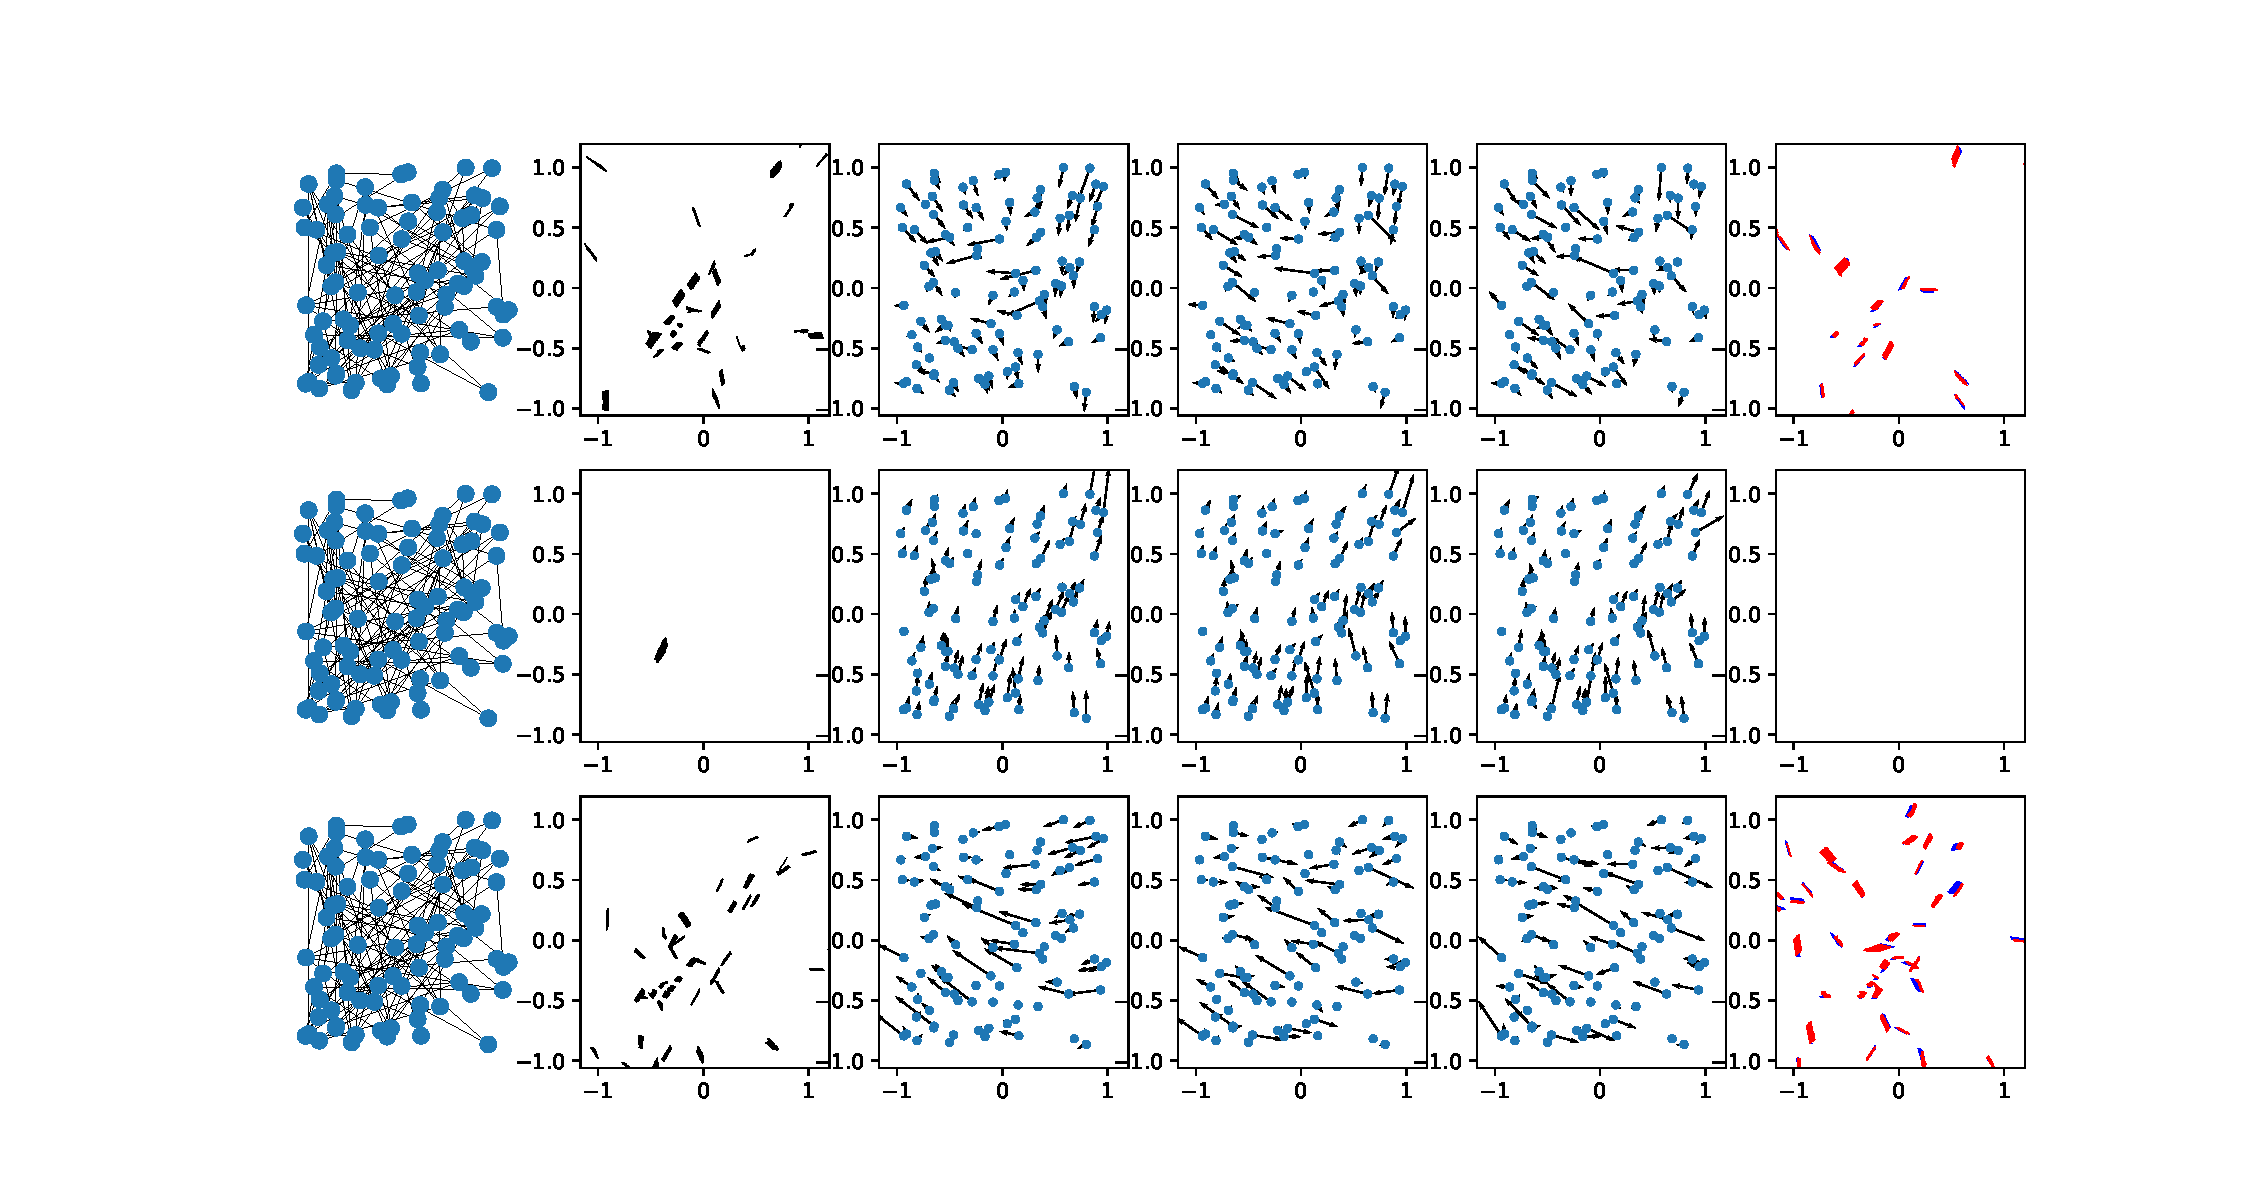
\includegraphics[trim={0 13.2cm 29.35cm 0},clip,width=\textwidth]{../results/rn1-100N-noemb-fixed}
    \caption{Random network with $p=1\%$}
  \end{subfigure}
  \begin{subfigure}{0.24\textwidth}
    \centering
    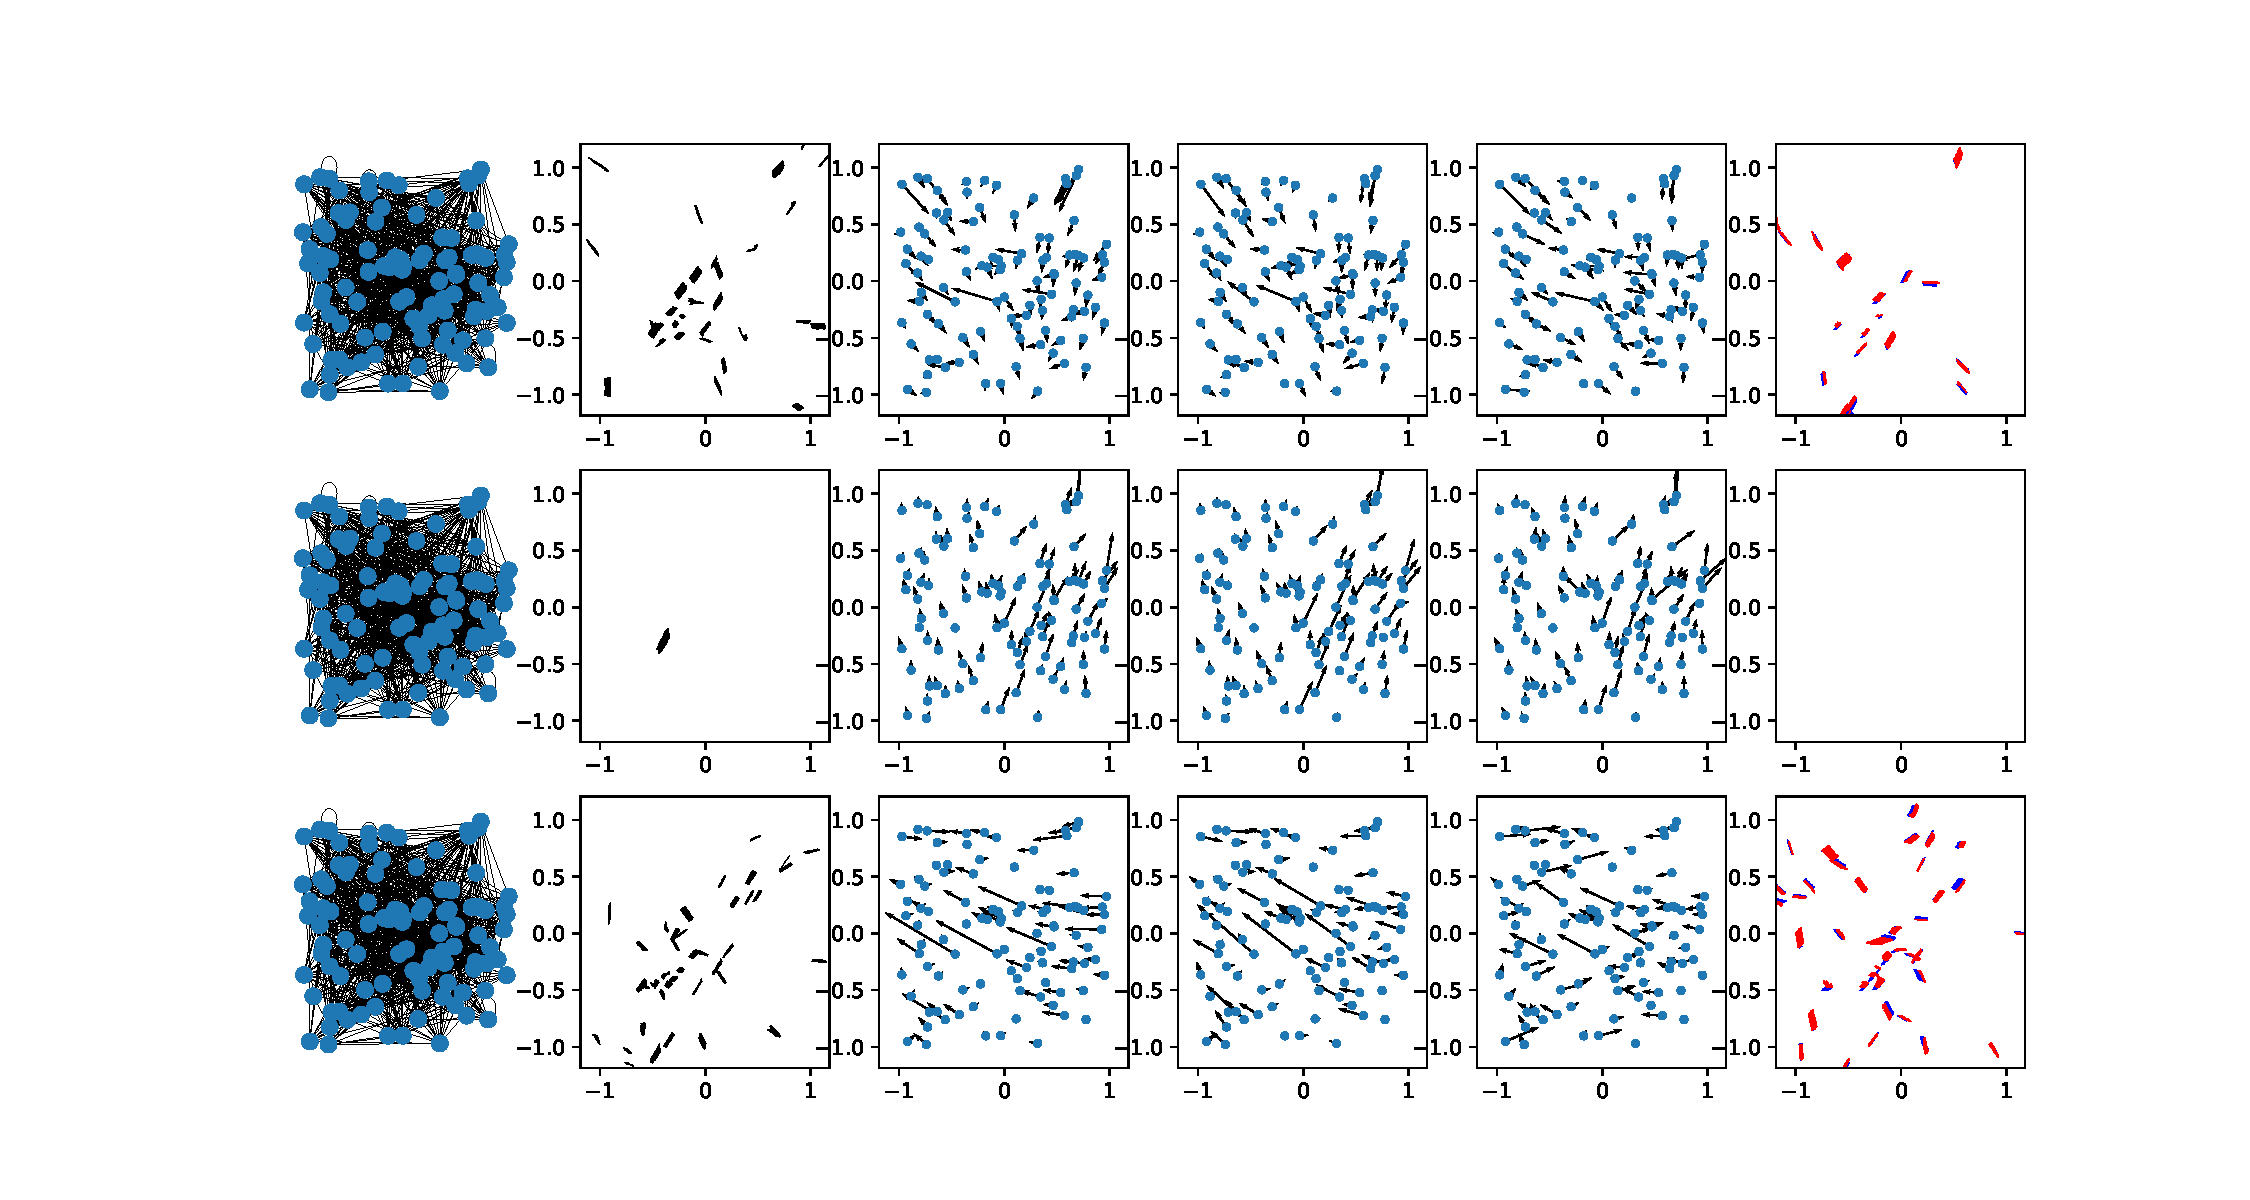
\includegraphics[trim={0 13.2cm 29.35cm 0},clip,width=\textwidth]{../results/rn10-100N-noemb-fixed}
    \caption{Random network with $p=10\%$}
  \end{subfigure}
  \begin{subfigure}{0.24\textwidth}
    \centering
    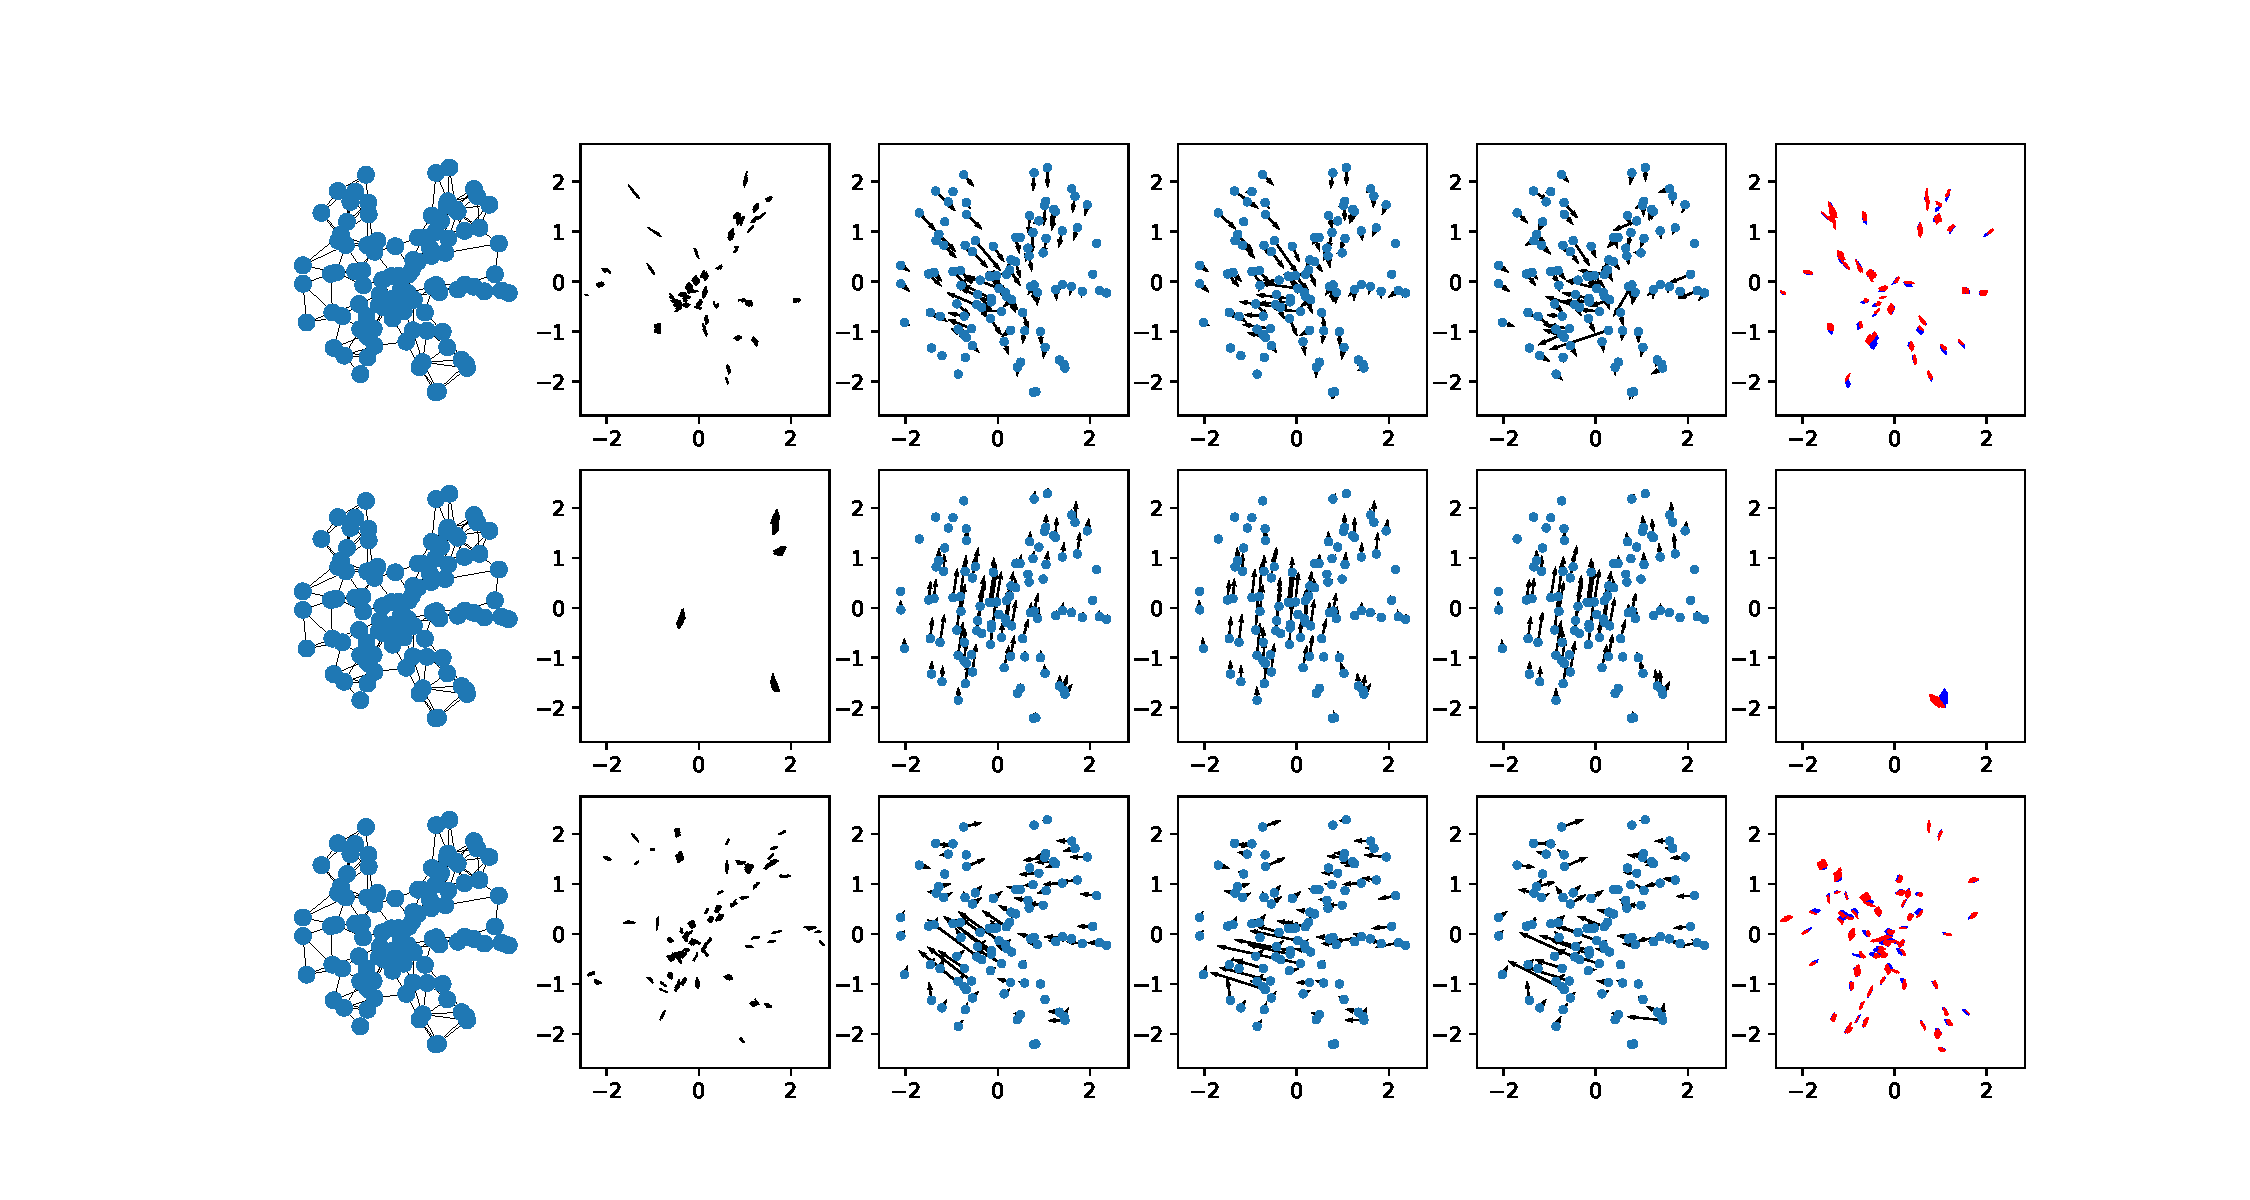
\includegraphics[trim={0 13.2cm 29.35cm 0},clip,width=\textwidth]{../results/nn-100N-noemb-fixed}
    \caption{$k$-means, 3nn}
  \end{subfigure}
  \begin{subfigure}{0.24\textwidth}
    \centering
    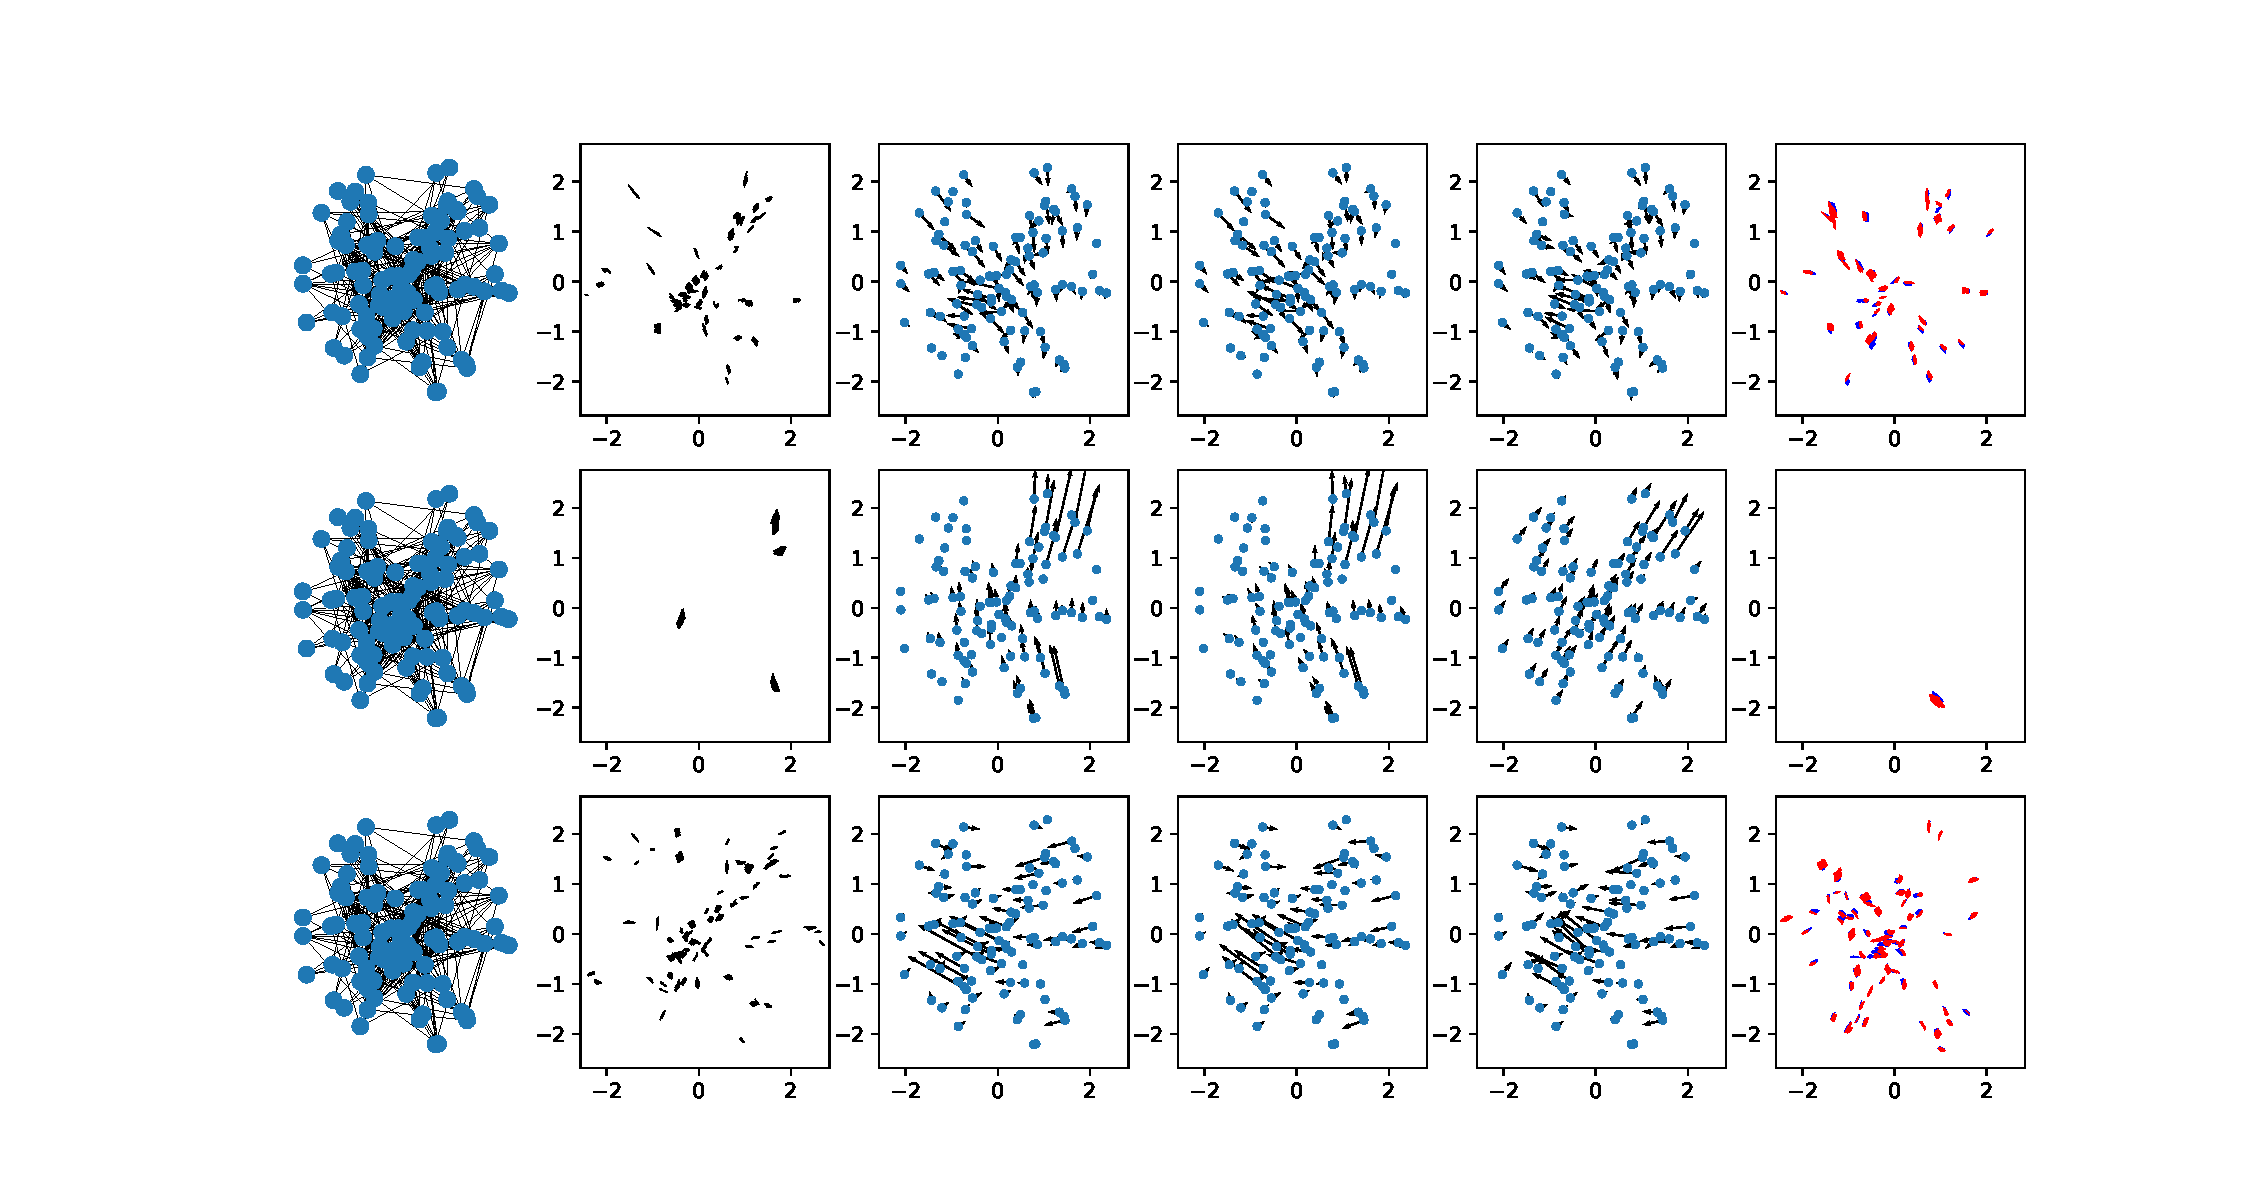
\includegraphics[trim={0 13.2cm 29cm 0},clip,width=\textwidth]{../results/ba-100N-noemb-fixed}
    \caption{$k$-means, BA}
  \end{subfigure}
  \begin{subfigure}{0.24\textwidth}
    \centering
    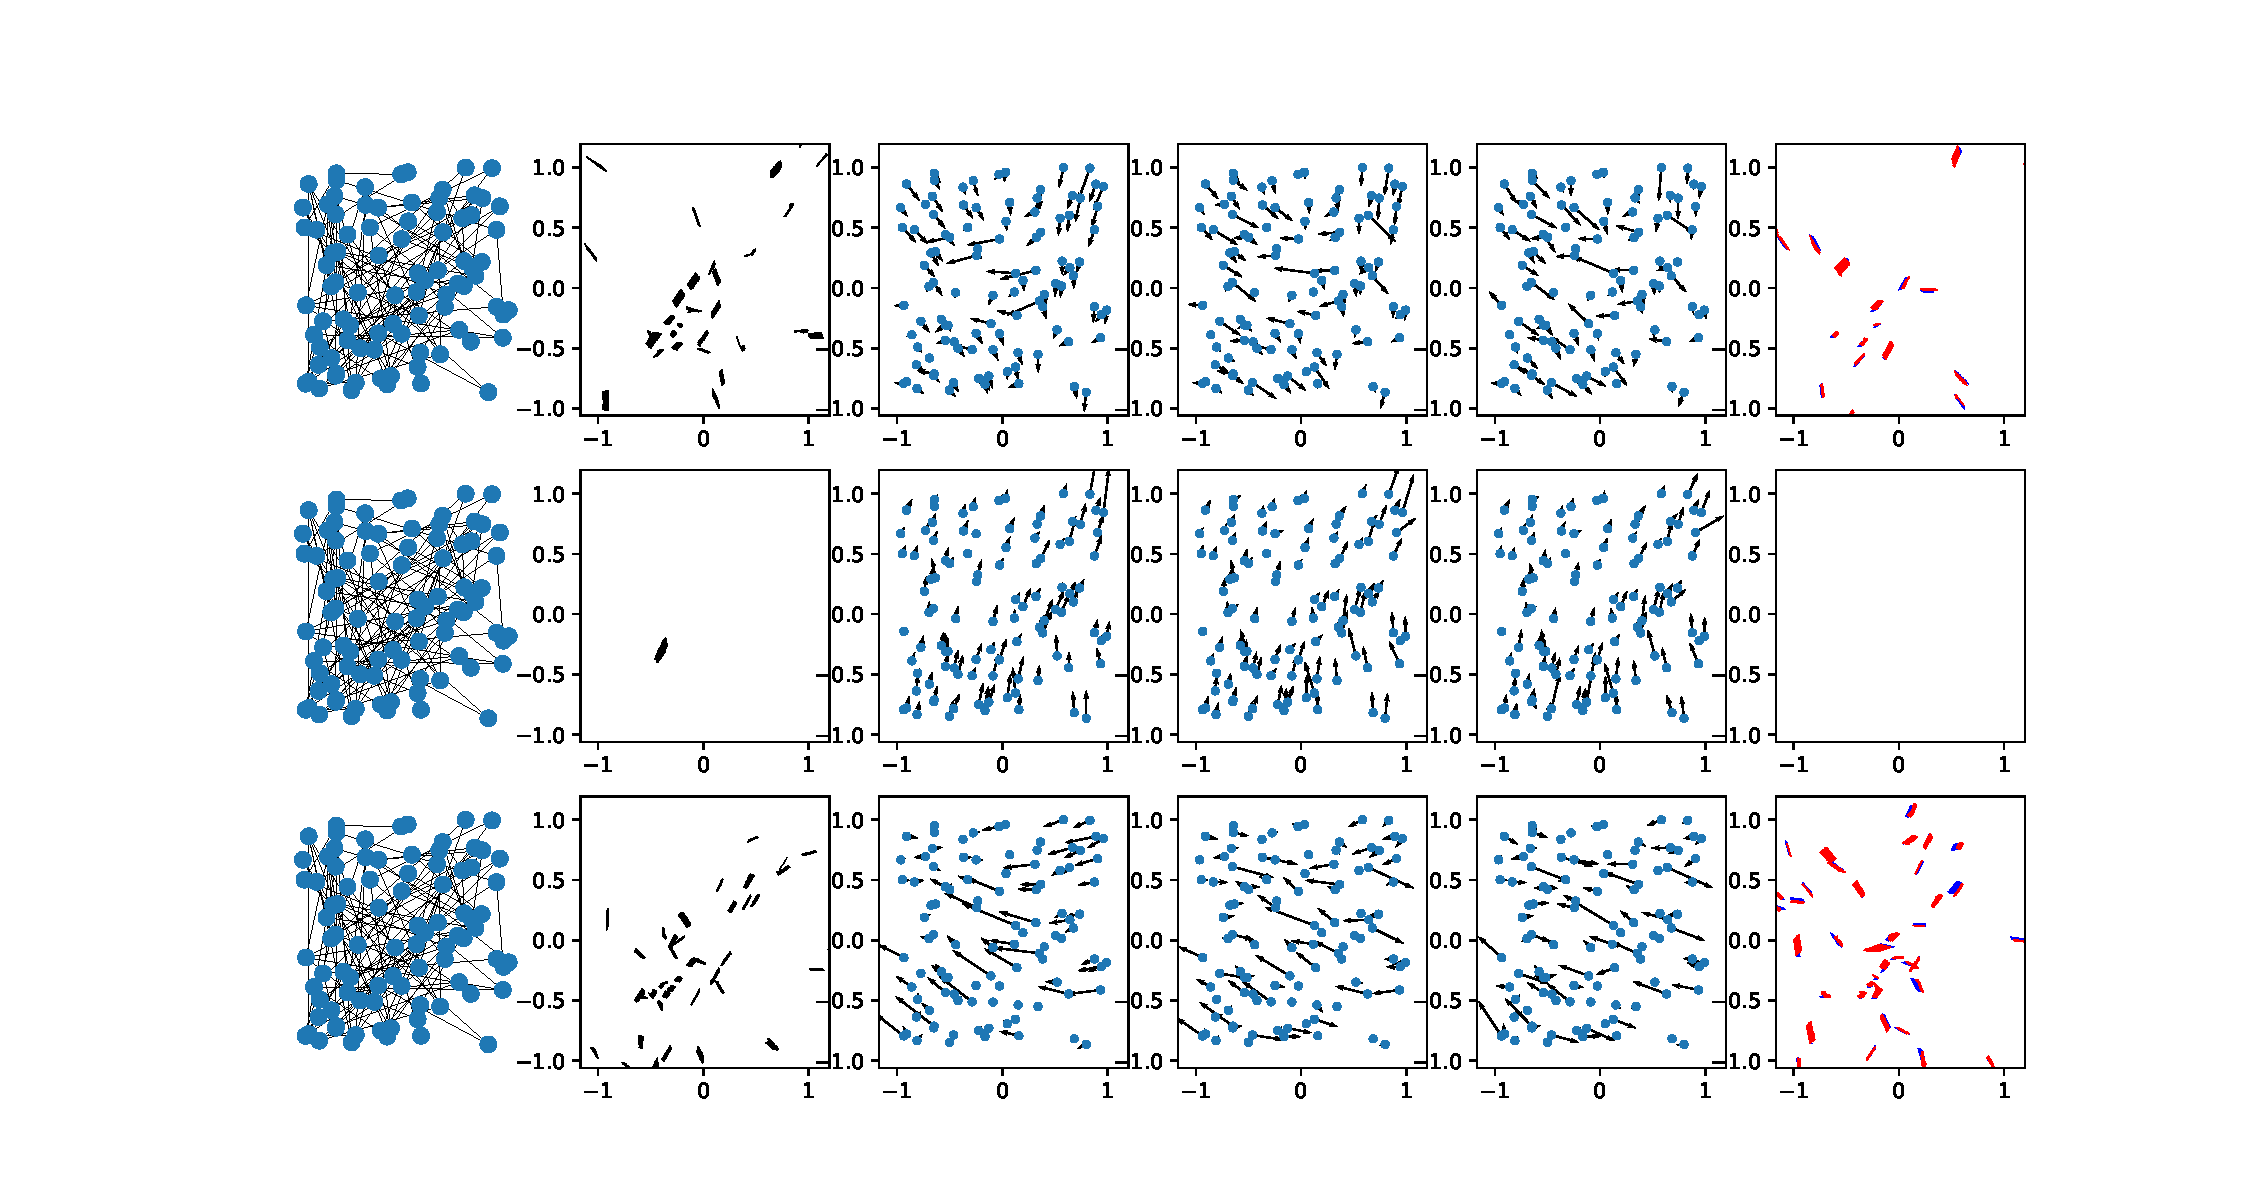
\includegraphics[trim={0 13.2cm 29cm 0},clip,width=\textwidth]{../results/rn1-100N-noemb0}
    \caption{Random network with $p=1\%$}
  \end{subfigure}
  \begin{subfigure}{0.24\textwidth}
    \centering
    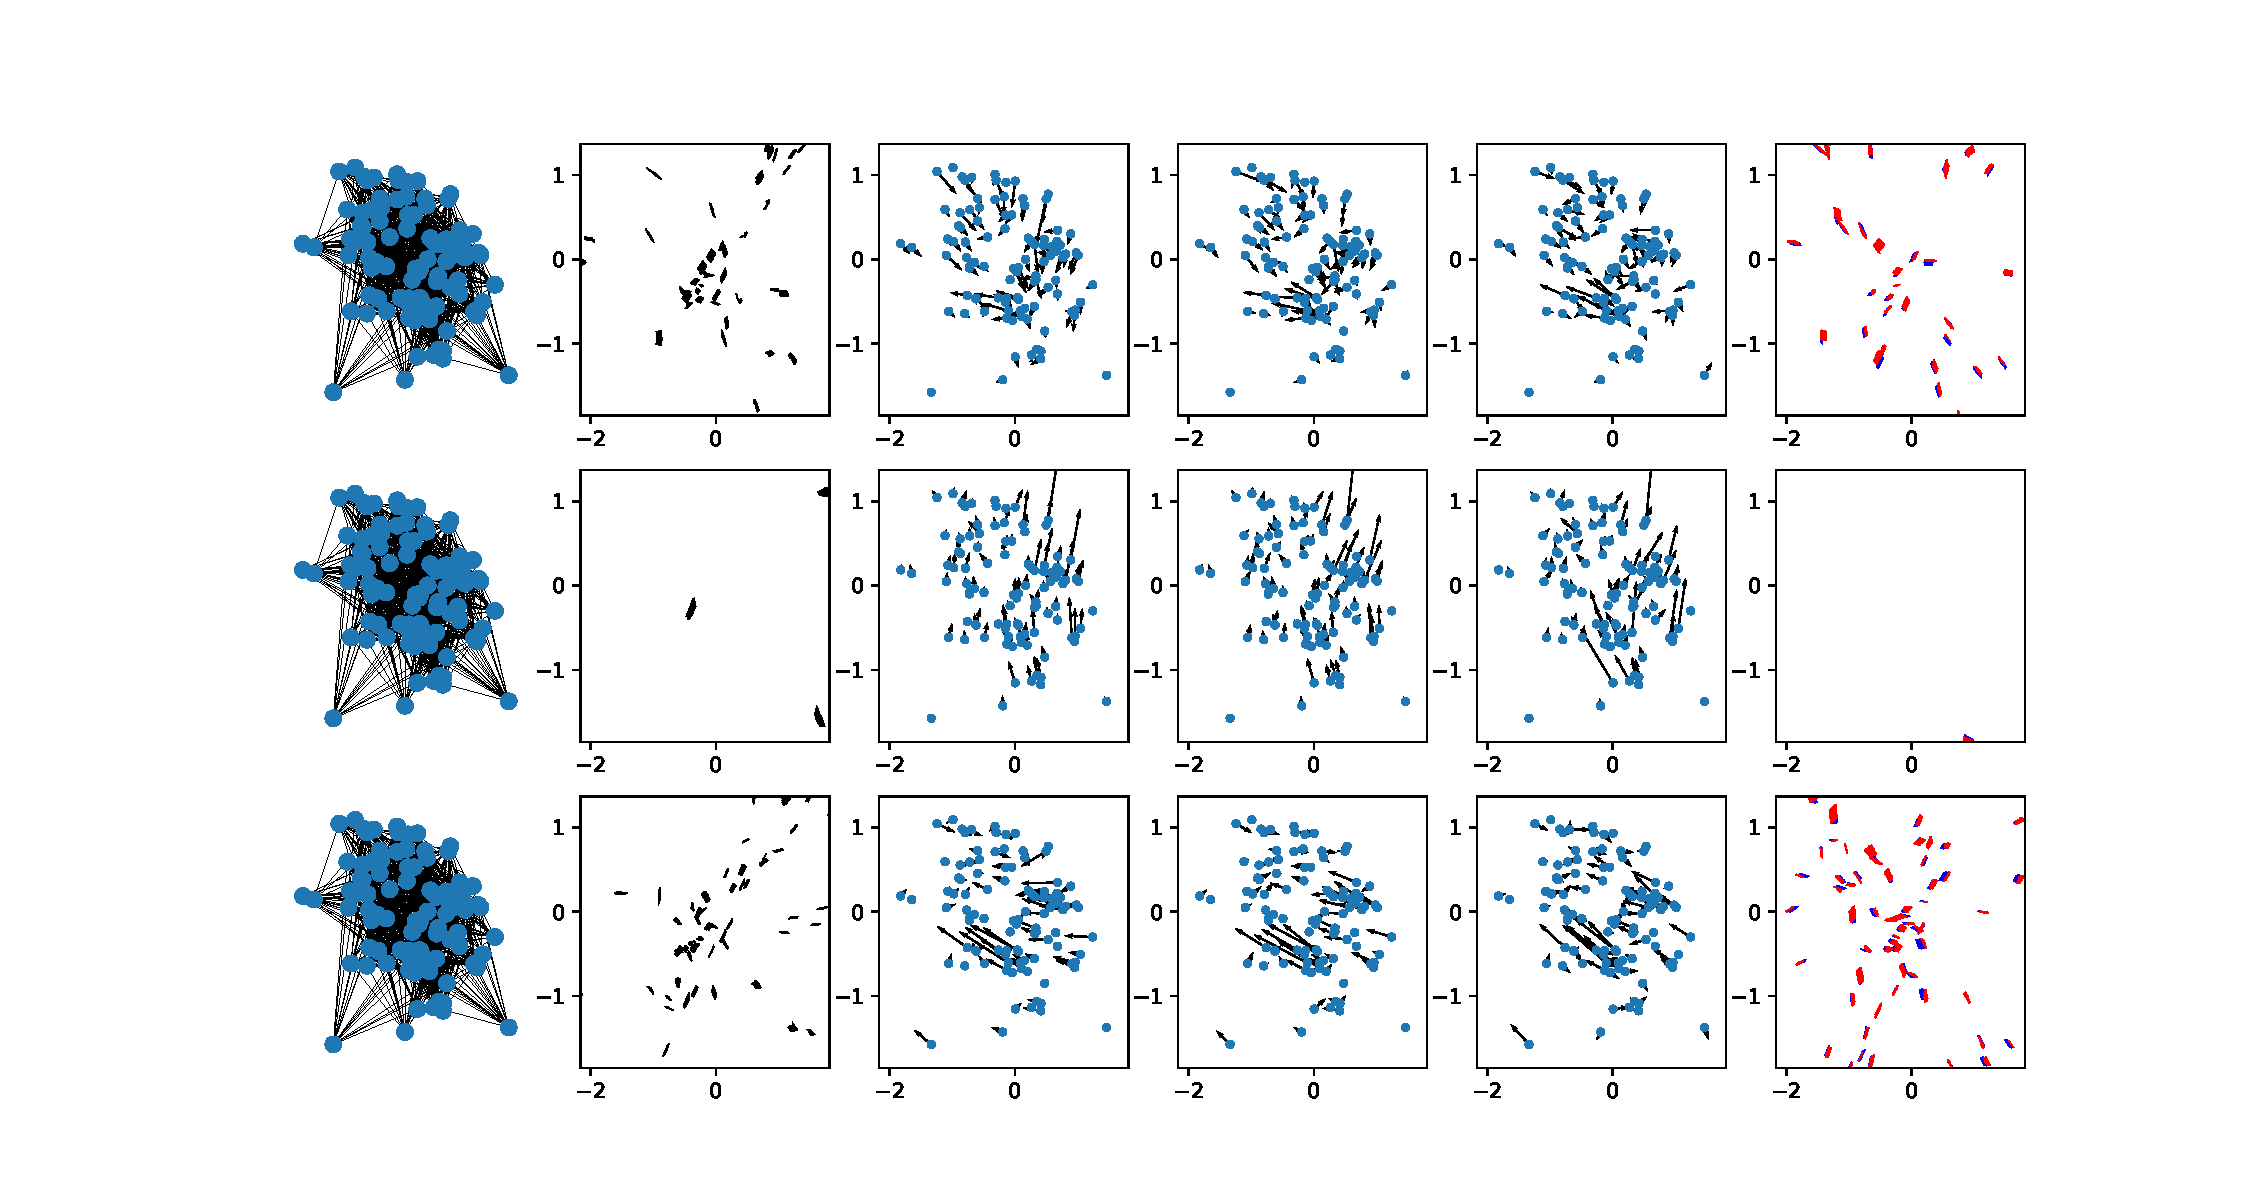
\includegraphics[trim={0 13.2cm 29cm 0},clip,width=\textwidth]{../results/rn10-100N-noemb0}
    \caption{Random network with $p=10\%$}
  \end{subfigure}
  \begin{subfigure}{0.24\textwidth}
    \centering
    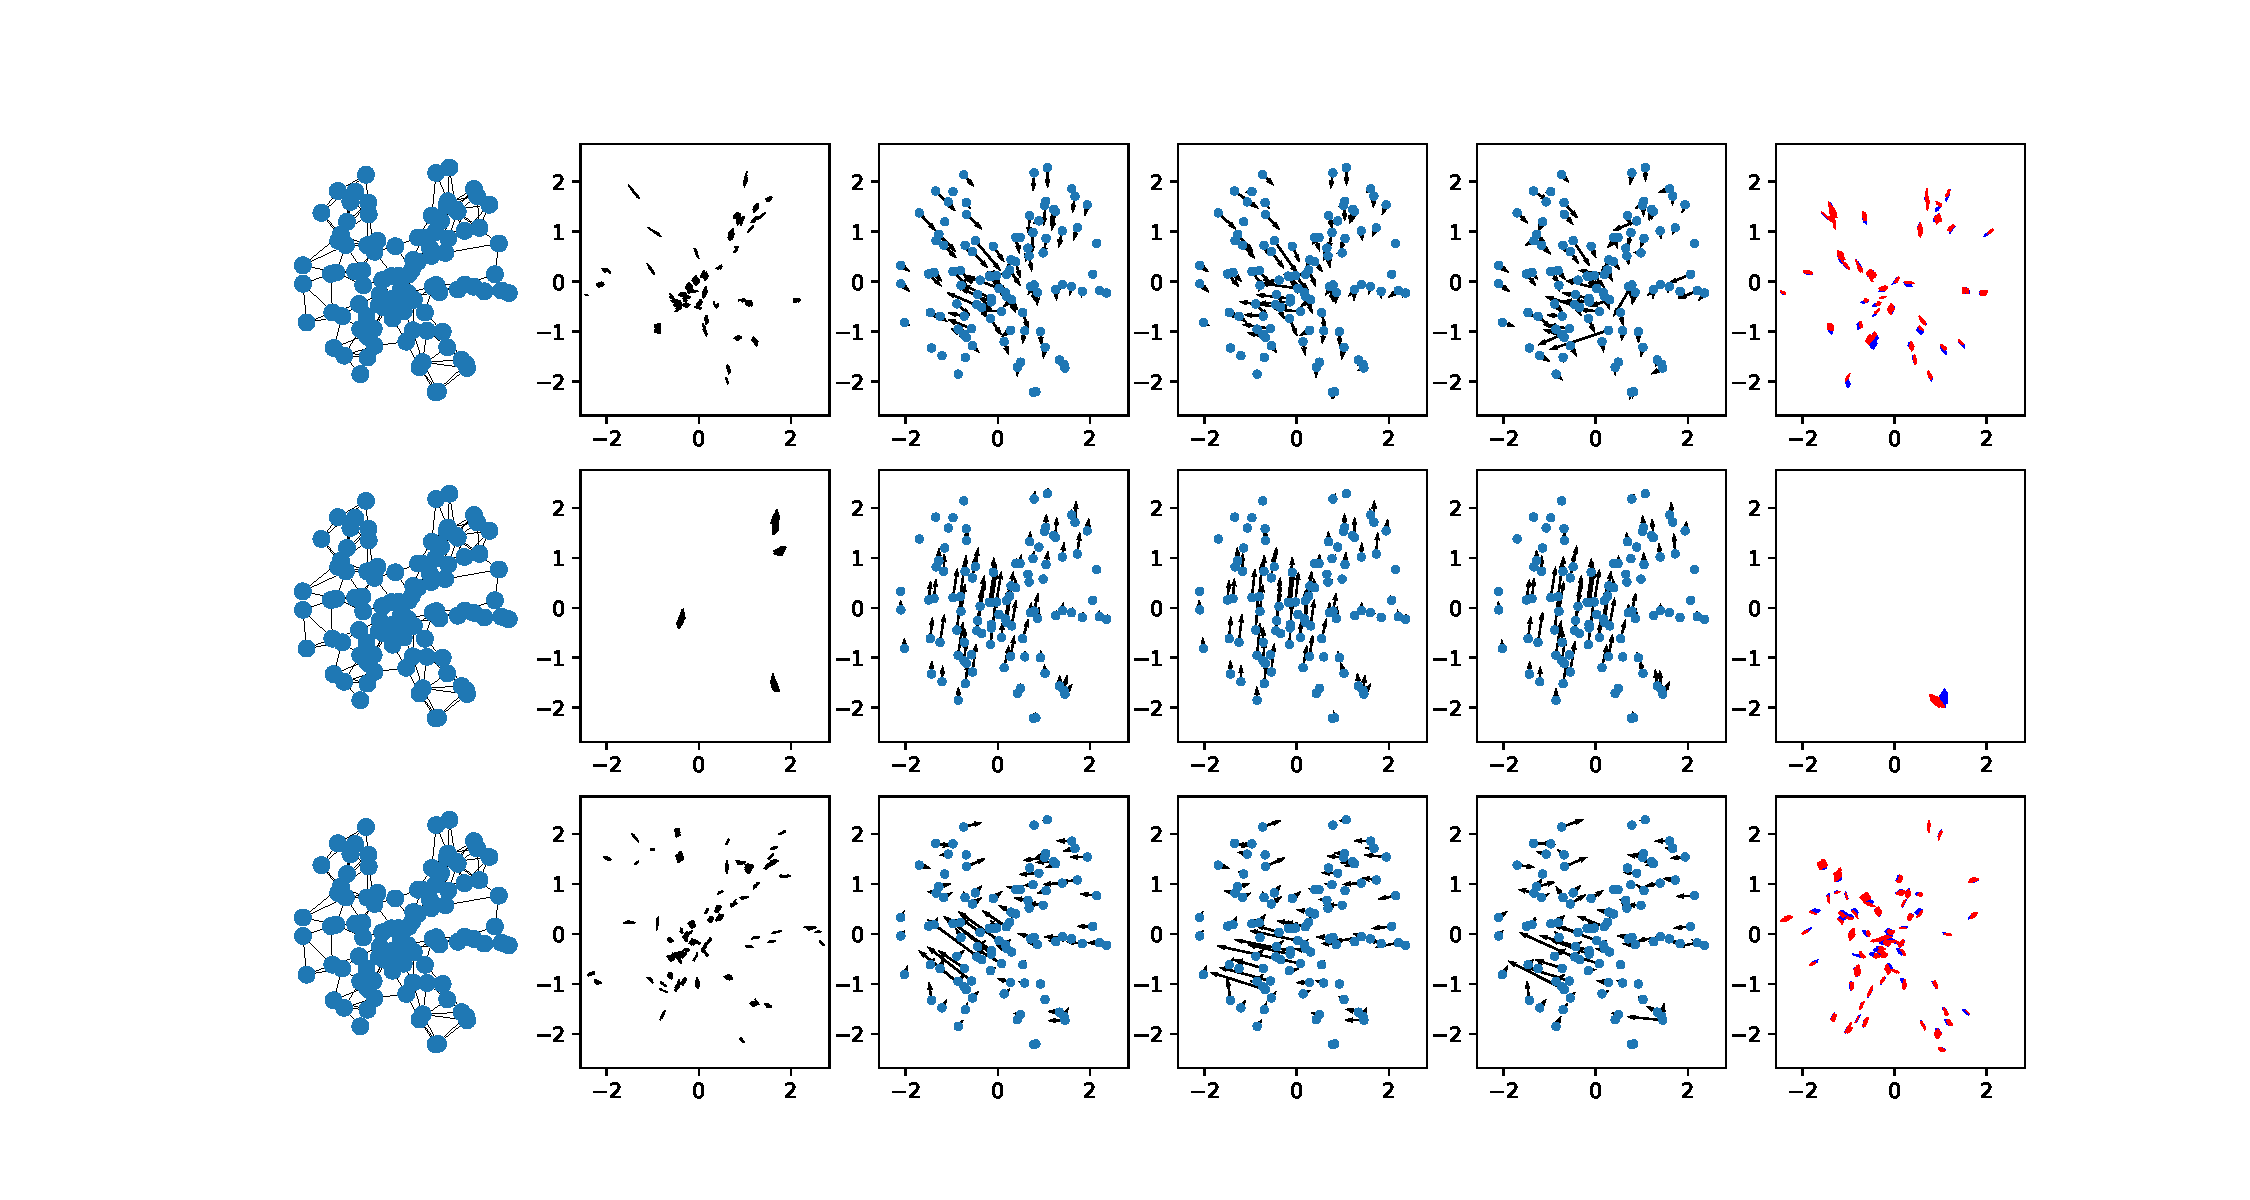
\includegraphics[trim={0 13.2cm 29cm 0},clip,width=\textwidth]{../results/nn-100N-noemb0}
    \caption{$k$-means, 3nn}
  \end{subfigure}
  \begin{subfigure}{0.24\textwidth}
    \centering
    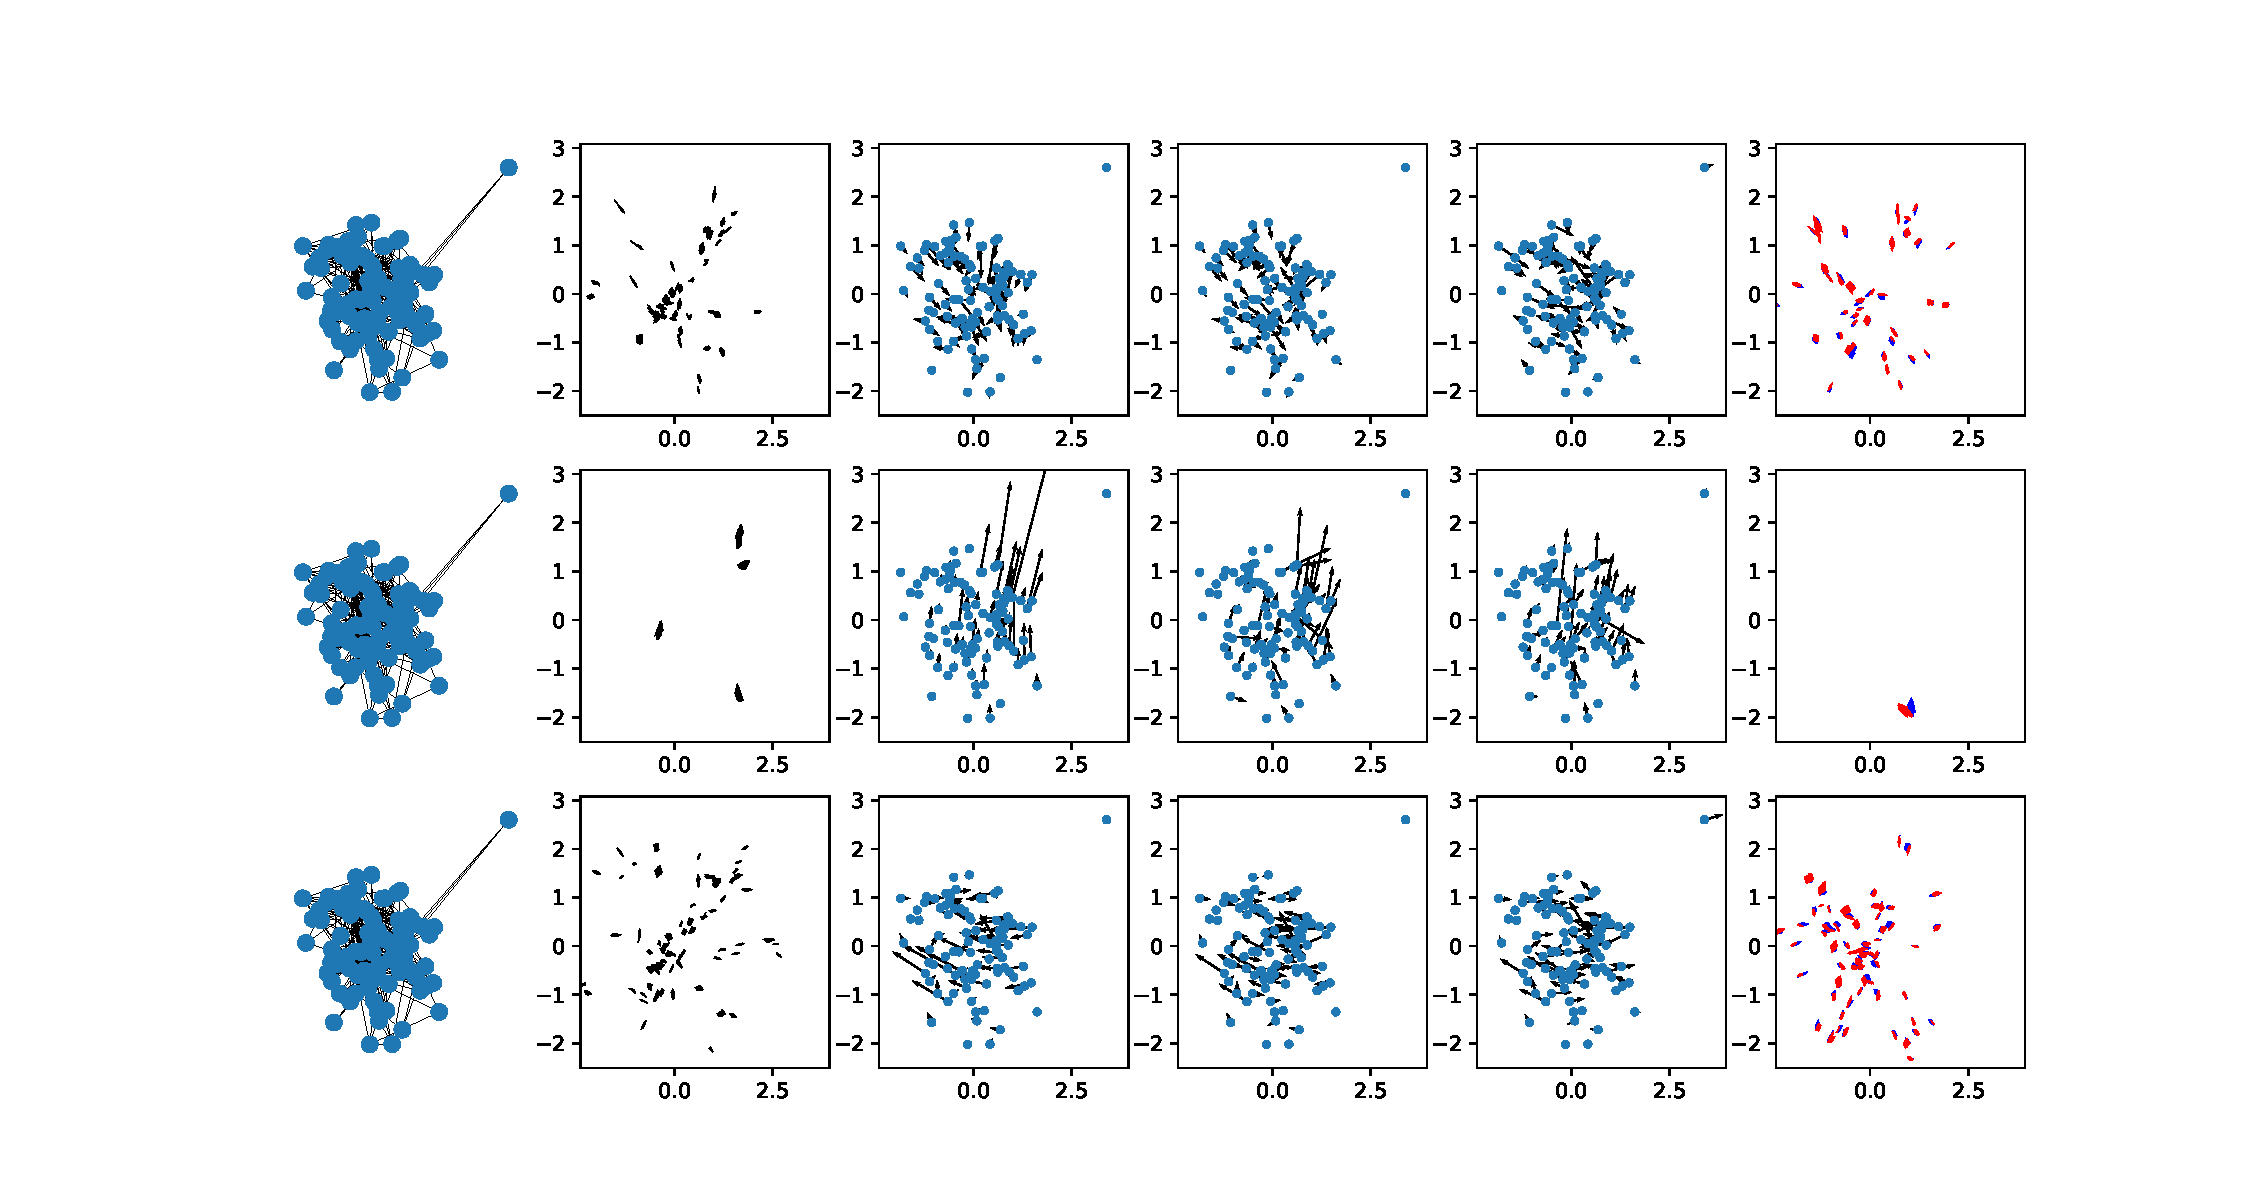
\includegraphics[trim={0 13.2cm 29cm 0},clip,width=\textwidth]{../results/ba-100N-noemb0}
    \caption{$k$-means, BA}
  \end{subfigure}
  \caption{Graph structure for the different models. The first row show graphs where each node has a fixed position, in the second row we see how this position has evolved during training.}
\end{figure}


\subsection{Nodes features}

\begin{table*}
  \label{tab:nodes}
  \centering
  \begin{tabular}{lcccc} \toprule
    \multirow{2}{*}{\textbf{Model}}                &                            & \multicolumn{3}{c}{\textbf{Nodes}}                                                          \\ \cmidrule(lr){3-5}
                                                   &                            & 10                                 & 100                   & 1000                           \\ \hline
    \multirow{2}{*}{\textbf{No Emb}}               & \scriptsize \textsc{Fixed} & 0.68 \tiny $\pm$ 0.01              & 0.69 \tiny $\pm$ 0.02 & 0.68 \tiny $\pm$ 0.01          \\
                                                   & \scriptsize \textsc{Adapt} & 0.68 \tiny $\pm$ 0.01              & 0.66 \tiny $\pm$ 0.01 & 0.65 \tiny $\pm$ 0.01          \\
    \multirow{2}{*}{\textbf{MLP}}                  & \scriptsize \textsc{Fixed} & 0.66 \tiny $\pm$ 0.01              & 0.66 \tiny $\pm$ 0.02 & 0.67 \tiny $\pm$ 0.02          \\
                                                   & \scriptsize \textsc{Adapt} & 0.XX \tiny $\pm$ 0.XX              & 0.XX \tiny $\pm$ 0.XX & 0. \tiny $\pm$ 0.              \\
    \multirow{2}{*}{\textbf{Added Pos-Enc + MLP}}  & \scriptsize \textsc{Fixed} & 1.03 \tiny $\pm$ 0.04              & 1.06 \tiny $\pm$ 0.02 & 1.04 \tiny $\pm$ 0.02          \\
                                                   & \scriptsize \textsc{Adapt} & 0.XX \tiny $\pm$ 0.XX              & 0.XX \tiny $\pm$ 0.XX & \textbf{0.00 \tiny $\pm$ 0.00} \\
    \multirow{2}{*}{\textbf{Concat Pos-Enc + MLP}} & \scriptsize \textsc{Fixed} & 0.65 \tiny $\pm$ 0.01              & 0.63 \tiny $\pm$ 0.01 & 0.65 \tiny $\pm$ 0.02          \\
                                                   & \scriptsize \textsc{Adapt} & 0.XX \tiny $\pm$ 0.XX              & 0.XX \tiny $\pm$ 0.XX & 0.XX \tiny $\pm$ 0.            \\

    \bottomrule
  \end{tabular}
  \caption{
    We tried different types of nodes embeddings for our model. The first one, is the baseline is to use no embedding layer and keep the aggregated wind value as the node state. The second one use a small MLP encoder to project the wind value to an higher dimensional space. Finally we explored two version of positional encoding layer. The results are the MSE error on the validation set, we ran ten different seeds to get the standard deviation. all measures are normalized.
  }
\end{table*}


Have a good baseline.



\section{Communication}
% (30 points)


\begin{itemize}
  \item Good report
  \item Github
  \item Streamlit
\end{itemize}

\section{Conclusion}

\bibliographystyle{apalike}
\bibliography{main}

\end{document}